\باب{برقی و مقناطیسی امواج}
لامحدود خطہ جس کا کوئی سرحد نہ ہو میں میکس ویل مساوات کا حل سادہ ترین مسئلہ ہے البتہ اس سے حاصل نتائج انتہائی دلچسپ اور معلوماتی ثابت ہوتے ہیں۔آپ دیکھیں گے کہ وقت کے ساتھ بدلتا برقی میدان، وقت کے ساتھ بدلتے مقناطیسی میدان کو جنم دیتا ہے جبکہ وقت کے ساتھ بدلتا مقناطیسی میدان، وقت کے ساتھ بدلتے برقی میدان کو جنم دیتا ہے۔چونکہ برقی میدان چارج کی بدولت جبکہ مقناطیسی میدان برقی رو کی بدولت ہے لہٰذا چارج یا رو میں کسی بھی تبدیل سے  باہمی تعاون سے بدلتا برقی اور بدلتا مقناطیسی میدان یعنی \اصطلاح{برقی و مقناطیسی}\فرہنگ{برقی و مقناطیسی}\حاشیہب{electromagnetic}\فرہنگ{electromagnetic} موج پیدا ہوتی ہے۔ایسے امواج کی \اصطلاح{تعدد}\فرہنگ{تعدد}\حاشیہب{frequency}\فرہنگ{frequency} کا دارومدار چارج یا رو (یا دونوں) میں تبدیلی کی شرح پر منحصر ہے۔یوں \عددیء{\omega} \اصطلاح{زاویائی تعدد}\فرہنگ{تعدد!زاویائی}\حاشیہب{angular frequency}\فرہنگ{frequency!angular} پر سائن نما شکل میں ارتعاش کرتا چارج \عددیء{\omega} زاویائی تعدد کی سائن نما موج ہی پیدا کرتی ہے۔برقی و مقناطیسی امواج  روشنی کی رفتار سے حرکت کرتی ہیں۔انسانی آنکھ مخصوص تعدد کی برقی و مقناطیسی امواج دیکھنے کی صلاحیت رکھتی ہے۔برقی و مقناطیسی امواج کے تعدد کی وہ پٹی جو ہمیں نظر آتی ہیں \اصطلاح{روشنی}\فرہنگ{روشنی}\حاشیہب{light}\فرہنگ{light} کہلاتی ہے۔سائن نما موج کو اس کی تعدد \عددیء{f} یا \اصطلاح{دوری عرصے}\فرہنگ{دوری عرصہ}\حاشیہب{time period}\فرہنگ{times period} \عددیء{\lambda} سے بیان کیا جا سکتا ہے۔ ہم \عددیء{\SI{380}{\nano\meter}} تا \عددیء{\SI{750}{\nano\meter}} کے دوری عرصے کے برقی و مقناطیسی امواج دیکھ سکتے ہیں۔

دو اشیاء کے سرحد پر برقی و مقناطیسی موج پر غور کرنے سے  شعاعی \اصطلاح{انعکاس}\فرہنگ{انعکاس}\حاشیہب{reflection}\فرہنگ{reflection}، شعاعی \اصطلاح{انحراف}\فرہنگ{انحراف}\حاشیہب{refraction}\فرہنگ{refraction} اور \اصطلاح{انکسار امواج}\فرہنگ{انکسار امواج}\فرہنگ{موج!انکسار}\حاشیہب{diffraction}\فرہنگ{diffraction}  کے حقائق دریافت ہوتے ہیں۔مختصراً شعاع کے تمام خصوصیات میکس ویل کے مساوات سے حاصل کرنا ممکن ہے۔

\حصہ{خالی خلاء میں برقی و مقناطیسی امواج}
جیسا کہ آپ جانتے ہیں کہ کسی بھی موصل یا نیم موصل کے اندر کسی طرح بھی پہنچایا گیا آزاد چارج جلد سطح پر پہنچ جاتا ہے۔اگر ہم ان لمحات کو نظر انداز کریں جتنی دیر میں آزاد چارج سطح تک نہیں پہنچ جاتا تو ہم ان اشیاء میں \عددیء{\rho_h=0} تصور کر سکتے ہیں۔ایسا ہی تصور کرتے ہوئے صفحہ \حوالہصفحہ{حصہ_میکس_ویل_میکس_ویل_نقطہ_اشکال} پر دئے گئے میکس ویل مساوات یہاں دوبارہ پیش کئے جاتے ہیں
\begin{align}
\nabla \times \kvec{E}&=-\mu \frac{\partial \kvec{H}}{\partial t}  \label{مساوات_موج_میکس_ویل_خالی_خلاء_الف}\\
\nabla \times \kvec{H}&=\sigma \kvec{E}+\epsilon \frac{\partial \kvec{E}}{\partial t}  \label{مساوات_موج_میکس_ویل_خالی_خلاء_ب}\\
\nabla \cdot \kvec{E}&=0 \label{مساوات_موج_میکس_ویل_خالی_خلاء_پ}\\
\nabla \cdot \kvec{H}&=0  \label{مساوات_موج_میکس_ویل_خالی_خلاء_ت}
\end{align}
جہاں \عددیء{\kvec{D}=\epsilon \kvec{E}} اور \عددیء{\kvec{B}=\mu \kvec{H}} کے علاوہ قانون اوہم کی نقطہ شکل \عددیء{\kvec{J}=\sigma \kvec{E}} کے  استعمال سے تمام مساوات صرف دو متغیرات \عددیء{\kvec{E}} اور \عددیء{\kvec{H}} کی صورت میں لکھے گئے ہیں۔

اس سے پہلے کہ ہم ان مساوات کو حل کریں، آئیں انہیں صرف دیکھ کر فیصلہ کریں کہ خالی خلاء میں ان سے  کیا نتائج اخذ کئے جا سکتے ہیں۔خالی خلاء میں کثافت برقی رو \عددیء{\kvec{J}}  صفر کے برابر ہوتی ہے۔اس حقیقت کو مد نظر رکھتے ہوئے آگے بڑھتے ہیں۔مساوات \حوالہ{مساوات_موج_میکس_ویل_خالی_خلاء_الف} کہتی ہے کہ کسی بھی نقطے پر مقناطیسی میدان میں وقت کے ساتھ تبدیلی سے اس نقطے کے گرد برقی میدان کی گردش پیدا ہوتی ہے۔گردش سے مراد ایسا میدان ہے جو بند دائرے پر اس نقطے کے گرد گھومتی ہو۔اگر مقناطیسی میدان کی قیمت زیادہ ہو تب برقی گردش کی قیمت بھی زیادہ ہو گی اور اگر مقناطیسی میدان کی قیمت کم ہو تب گردش بھی کم ہو گی۔یوں دو حقائق سامنے آتے ہیں۔پہلی حقیقت یہ ہے کہ کسی بھی نقطے پر بدلتا مقناطیسی میدان اس نقطے کے گرد، یعنی نقطے سے ذرہ دور، برقی میدان پیدا کرتی ہے اور دوسری حقیقت یہ کہ پہلی میدان کی قیمت کم یا زیادہ کرنے سے پیدا میدان کی قیمت بھی تبدیل ہوتی ہے یعنی بدلتا مقناطیسی میدان، بدلتے برقی میدان کو جنم دیتا ہے۔اسی طرح مساوات \حوالہ{مساوات_موج_میکس_ویل_خالی_خلاء_ب} کہتی ہے کہ کسی بھی نقطے پر برقی میدان میں وقت کے ساتھ تبدیلی سے اس نقطے کے گرد مقناطیسی گردش پیدا ہوتی ہے۔یہاں بھی صاف واضح ہے کہ کسی بھی نقطے پر برقی میدان میں وقت کے ساتھ تبدیل، اس نقطے سے ذرہ دور، بدلتی مقناطیسی میدان پیدا کرتی ہے۔ایسا معلوم ہوتا ہے کہ بدلتا مقناطیسی میدان کچھ فاصلے پر آگے کر کے بدلتا برقی میدان پیدا کرتا ہے جو مزید آگے مقناطیسی میدان پیدا کرتا ہے اور یہ سلسلہ چلے جاتا ہے۔جیسا کہ ہم جلد دیکھیں گے، ایسے جڑواں، ہاتھ میں ہاتھ ڈالے، حرکت کرتے بدلتے برقی اور بدلتے مقناطیسی میدان کی رفتار \عددیء{\tfrac{1}{\sqrt{\epsilon_0 \mu_0}}} یعنی تقریباً \عددیء{\SI{3e8}{\meter \per \second}} ہے جو خالی خلاء میں روشنی کی رفتار ہے۔

\حصہ{برقی و مقناطیسی امواج}
میکس ویل مساوات کے حل \اصطلاح{دوری سمتیات}\فرہنگ{دوری سمتیہ}\حاشیہب{phasor}\فرہنگ{phasor} کی مدد سے نہایت آسان ہو جاتے ہیں لہٰذا پہلے دوری سمتیہ پر غور کرتے ہیں جو آپ نے برقی ادوار حل کرتے وقت ضرور استعمال کئے ہوں گے۔

سائن نما لہر کی عمومی شکل 
\begin{align}\label{مساوات_موج_اصل_سائن_نما_تفاعل}
E_y =E_{xyz} \cos (\omega t +\psi)
\end{align} 
ہے جہاں
\begin{align}
\omega =2\pi f
\end{align}
\اصطلاح{زاویائی تعدد}\فرہنگ{تعدد!زاویائی}\فرہنگ{زاویائی!تعدد}\حاشیہب{angular frequency}\فرہنگ{angular frequency} اور \عددیء{\phi} \اصطلاح{زاویائی فاصلہ}\فرہنگ{زاویائی فاصلہ}\حاشیہب{phase angle}\فرہنگ{phase angle} ہیں جبکہ \عددیء{E_{xyz}} ازخود \عددیء{x}، \عددیء{y}، \عددیء{z} اور \عددیء{\omega} کا \اصطلاح{تابع تفاعل}\فرہنگ{تابع تفاعل}\فرہنگ{تفاعل!تابع}\حاشیہب{dependent function}\فرہنگ{function!dependent} ہو سکتا ہے۔تعدد \عددیء{f} کی اکائی \اصطلاح{ہرٹز}\فرہنگ{ہرٹز}\حاشیہب{Hertz}\فرہنگ{Hertz} ہے۔یہاں دھیان رہے کہ \عددیء{E_{xyz}} وقت \عددیء{t} کا تابع نہیں ہے۔

کسی بھی متغیرہ \عددیء{x} کے لئے \اصطلاح{یولر مماثل}\فرہنگ{یولر مماثل}\حاشیہب{Euler's identity}\فرہنگ{Euler's identity}  کو \عددیء{e^{j x}=\cos x +j \sin x} لکھا جاتا ہے جہاں \عددیء{j=\sqrt{-1}} \اصطلاح{خیالی عدد}\فرہنگ{خیالی!عدد}\حاشیہب{imaginary number}\فرہنگ{imaginary!number} ہے ۔آزاد متغیرہ \عددیء{\omega t +\psi} کے لئے یولر مماثل
\begin{align*}
e^{j (\omega t +\psi)}=\cos (\omega t +\psi) +j \sin (\omega t +\psi)
\end{align*}
لکھا جا سکتا ہے جو \اصطلاح{حقیقی}\فرہنگ{حقیقی}\حاشیہب{real}\فرہنگ{real} اور \اصطلاح{خیالی}\فرہنگ{خیالی}\حاشیہب{imaginary}\فرہنگ{imaginary} اجزاء پر مشتمل  \اصطلاح{مخلوط تفاعل}\فرہنگ{مخلوط تفاعل}\فرہنگ{تفاعل!مخلوط}\حاشیہب{complex function}\فرہنگ{function!complex} ہے۔یوں \عددیء{\cos (\omega t +\psi)} کو \عددیء{e^{j(\omega t +\psi)}} کا حقیقی جزو تصور کیا جا سکتا ہے۔اس طرح
\begin{align*}
E_y=E_{xyz} \cos (\omega t +\psi)= \left[E_{xyz} e^{j(\omega t +\psi)}\right]_{\textrm{حقیقی}}= \left[E_{xyz} e^{j \omega t }e^{j\psi}\right]_{\textrm{حقیقی}}
\end{align*}
لکھا جا سکتا ہے جہاں زیر نوشت میں \عددیء{\textrm{حقیقی}} لکھنے سے مراد یہ ہے کہ پورے تفاعل کا حقیقی جزو لیا جائے۔مندرجہ بالا مساوات کو بطور دوری سمتیہ یوں
\begin{align*}
E_{ys} =E_{xyz} e^{j \psi}
\end{align*}
 لکھا جاتا ہے جہاں  \عددیء{e^{j \omega t}} اور زیر نوشت میں \عددیء{\textrm{حقیقی}} کو پوشیدہ رکھا جاتا ہے۔ اس مساوات کے بائیں ہاتھ \عددیء{E_{ys}} لکھتے ہوئے زیر نوشت میں \عددیء{s} یاد دلاتی ہے کہ یہ مساوات دوری سمتیہ کی شکل میں لکھی گئی ہے لہٰذا یاد رہے کہ اصل تفاعل میں \عددیء{e^{j \omega t}} پایا جاتا ہے اور پورے تفاعل کا صرف حقیقی جزو ہی لیا جائے۔تفاعل \عددیء{E_{ys}} کے زیر نوشت میں \عددیء{s} دراصل اس حقیقت کو ظاہر کرتی ہے کہ  اس تفاعل کا آزاد متغیرہ،  \اصطلاح{مخلوط تعدد}\فرہنگ{تعدد!مخلوط}\فرہنگ{مخلوط!تعدد}\حاشیہب{complex frequency}\فرہنگ{complex!frequency}\فرہنگ{frequency!complex} ہے۔ہمارے استعمال میں  \عددیء{s} خیالی عدد یعنی \عددیء{{s=j \omega}} ہو گا۔

اب \عددیء{E_y=10.5\cos(10^6 t -0.35z)} کو دوری سمتیہ کی شکل میں لکھنے کی خاطر اسے یولر مماثل کے حقیقی جزو
\begin{align*}
E_y=\left[10.5 e^{j(10^6 t -0.35z)} \right]_{\textrm{حقیقی}}=\left[10.5 e^{j10^6 t} e^{ -j0.35z} \right]_{\textrm{حقیقی}}
\end{align*}
لکھنے کے بعد \عددیء{e^{j10^6t}} اور زیر نوشت میں \عددیء{\textrm{حقیقی}} کو پوشیدہ رکھتے ہوئے یوں
\begin{align*}
E_{ys}=10.5 e^{-j 0.35z}
\end{align*} 
لکھا جائے گا جہاں بائیں ہاتھ \عددیء{E_{ys}} میں زیر نوشت میں \عددیء{s} کا اضافہ کیا گیا۔یاد رہے کہ \عددیء{E_y} حقیقی تفاعل ہے جبکہ \عددیء{E_{ys}} عموماً مخلوط تفاعل ہوتا ہے۔

دوری سمتیہ سے اصل تفاعل حاصل کرنے کی خاطر اسے \عددیء{e^{j \omega t}} سے ضرب دیتے ہوئے حاصل جواب کا حقیقی جزو لیا جاتا ہے۔

مساوات \حوالہ{مساوات_موج_اصل_سائن_نما_تفاعل} کا وقت کے ساتھ جزوی تفرق
\begin{align*}
\frac{\partial E_y}{\partial t}&=\frac{\partial }{\partial t} [E_{xyz} \cos(\omega t +\psi)]=-\omega E_{xyz} \sin (\omega t +\psi)\\
&=\left[j \omega  E_{xyz} e^{j(\omega t +\psi)} \right]_{\textrm{حقیقی}}
\end{align*} 
کے برابر ہے۔یہ عمومی نتیجہ ہے جس کے تحت وقت کے ساتھ تفاعل کا تفرق، دوری سمتیہ کو \عددیء{j \omega} سے ضرب دینے کے مترادف ہے۔یوں مثال کے طور پر اگر
\begin{align*}
\frac{\partial E_x}{\partial t}=-\frac{1}{\epsilon_0} \frac{\partial H_y}{\partial z}
\end{align*}
ہو تب اسی کی دوری سمتیہ شکل
\begin{align*}
j \omega E_{xs}=-\frac{1}{\epsilon_0} \frac{\partial H_y}{\partial z}
\end{align*}
ہو گی۔اسی طرح سائن نما میدان کے لئے میکس ویل کے مساوات بھی با آسانی دوری سمتیہ کی شکل میں لکھے جا سکتے ہیں لہٰذا
\begin{align*}
\nabla \times \kvec{E}=-\mu\frac{\partial \kvec{H}}{\partial t}
\end{align*} 
کو دوری سمتیہ کی صورت میں
\begin{align}   \label{مساوات_موج_میکس_ویل_دوری_سمتیہ_شکل_الف}
\nabla \times \kvec{E}_s=-j \omega \mu \kvec{H}_s
\end{align}
لکھا جائے گا۔میکس ویل کے بقایا مساوات کو بھی دوری سمتیہ کی صورت میں لکھتے ہیں۔
\begin{align}
\nabla \times \kvec{H}_s &=\left(\sigma +j \omega \epsilon \right) \kvec{E}_s   \label{مساوات_موج_میکس_ویل_دوری_سمتیہ_شکل_ب}\\
\nabla \cdot \kvec{E}_s &=0   \label{مساوات_موج_میکس_ویل_دوری_سمتیہ_شکل_پ}\\
\nabla \cdot \kvec{H}_s&=0   \label{مساوات_موج_میکس_ویل_دوری_سمتیہ_شکل_ت}
\end{align}

آئیں ان مساوات سے امواج کی مساوات حاصل کریں۔ایسا کرنے کی خاطر مساوات \حوالہ{مساوات_موج_میکس_ویل_دوری_سمتیہ_شکل_الف} کی گردش
\begin{align*}
\nabla \times \nabla \times \kvec{E}_s=\nabla \left(\nabla \cdot \kvec{E}_s \right)-\nabla^2 \kvec{E}_s=-j \omega \mu  \nabla \times \kvec{H}_s
\end{align*}
میں مساوات \حوالہ{مساوات_موج_میکس_ویل_دوری_سمتیہ_شکل_ب} اور مساوات \حوالہ{مساوات_موج_میکس_ویل_دوری_سمتیہ_شکل_پ} پر کرنے سے
\begin{align}\label{مساوات_موج_ہلم_ہولٹز_مساوات}
\nabla^2 \kvec{E}_s=j \omega \mu  \left(\sigma +j \omega \epsilon \right) \kvec{E}_s =\gamma^2 \kvec{E}_s
\end{align}
حاصل ہوتا ہے  جہاں 
\begin{align}\label{مساوات_موج_حرکی_مستقل_الف}
\gamma=\mp \sqrt{j \omega \mu  \left(\sigma +j \omega \epsilon \right)}
\end{align}
\اصطلاح{حرکی مستقل}\فرہنگ{حرکی مستقل}\حاشیہب{propagation constant}\فرہنگ{propagation constant} کہلاتا ہے۔چونکہ \عددیء{j \omega \mu (\sigma+j \omega \epsilon)} مخلوط عدد ہے لہٰذا اس کا جزر \عددیء{\gamma} بھی مخلوط عدد ہو گا جسے
\begin{align}
\gamma=\alpha+j \beta
\end{align}
لکھا جا سکتا ہے جہاں \عددیء{\alpha} اور \عددیء{\beta} مثبت اور حقیقی اعداد ہیں۔

 مساوات \حوالہ{مساوات_موج_ہلم_ہولٹز_مساوات}  \اصطلاح{سمتی ہلم ہولٹز} مساوات\فرہنگ{ہلم ہولٹز!سمتی مساوات}\حاشیہب{vector Helmholtz equation}\فرہنگ{Helmholtz!vector equation}\حاشیہد{ہرمن لڈوگ فرڈینانڈ ون ہلم ہولٹز جرمنی کے عالم طبیعیات تھے۔} کہلاتی ہے۔کارتیسی محدد میں بھی سمتی ہلم ہولٹز مساوات کی بڑی شکل  کافی خوفناک نظر آتی ہے چونکہ اس سے چار چار اجزاء پر مشتمل تین عدد مساوات نکلتے ہیں۔کارتیسی محدد میں اس  کی \عددیء{x} مساوات 
\begin{align}
\nabla^2 E_{xs}=\gamma^2 E_{xs} 
\end{align}
یعنی
\begin{align}
\frac{\partial^2  E_{xs}}{\partial x^2}+\frac{\partial^2  E_{xs}}{\partial y^2}+\frac{\partial^2  E_{xs}}{\partial z^2} =\gamma^2  E_{xs} 
\end{align}
ہے۔ہم فرض کرتے ہیں کہ جن امواج پر ہم غور کرنا چاہتے ہیں ان میں نا تو \عددیء{x} اور نا ہی \عددیء{y} کے ساتھ میدان تبدیل ہوتے ہیں۔ایسی صورت
 میں \عددیء{{\tfrac{\partial^2  E_{xs}}{\partial x^2}=0}} اور \عددیء{{\tfrac{\partial^2  E_{xs}}{\partial y^2}=0}} ہوں گے لہٰذا  مندرجہ بالا مساوات
\begin{align}
\frac{\partial^2  E_{xs}}{\partial z^2} =\gamma^2 E_{xs} 
\end{align}
صورت اختیار کر لے گی۔اس طرح کے دو درجی تفرقی مساوات آپ نے پڑھے ہوں گا لہٰذا میں توقع رکھتا ہوں کہ آپ اس کے حل
\begin{align}\label{مساوات_موج_مثبت_زیڈ_جانب}
E_{xs}&=A e^{-\gamma z}
\end{align}
اور
\begin{align}\label{مساوات_موج_منفی_زیڈ_جانب}
E_{xs}&=Be^{\gamma z}
\end{align}
لکھ سکتے ہیں۔

آئیں \عددیء{\gamma=\alpha+j\beta} پر کرتے ہوئے ان جوابات میں سے مساوات \حوالہ{مساوات_موج_مثبت_زیڈ_جانب} پر غور کریں۔مساوات \حوالہ{مساوات_موج_مثبت_زیڈ_جانب} درحقیقت دوری سمتیہ ہے لہٰذا اسے  \عددیء{e^{j\omega t}} سے ضرب دے کر
\begin{align*}
E_x&=\left[A e^{j \omega t} e^{-(\alpha+j \beta) z} \right]_{\textrm{حقیقی}}\\
&=\left[A e^{-\alpha z} e^{j(\omega t -\beta z)} \right]_{\textrm{حقیقی}}
\end{align*}
حقیقی  جزو
\begin{align*}
E_x=A e^{-\alpha z} \cos (\omega t -\beta z)
\end{align*}
لیتے ہیں۔مساوات کے مستقل \عددیء{A} کی جگہ \عددیء{t=0} اور \عددیء{z=0} پر میدان کی قیمت \عددیء{E_0} پر کرتے ہوئے اصل حل
\begin{align}\label{مساوات_موج_کوسائن_مثبت_موج}
E_x=E_0 e^{-\alpha z} \cos (\omega t -\beta z)
\end{align}
لکھا جا سکتا ہے۔یہ موج کی وہ مساوات  ہے جس کی تلاش میں ہم نکلے تھے۔اگر ہم مساوات \حوالہ{مساوات_موج_منفی_زیڈ_جانب} کو لے کر آگے بڑھتے تو مساوات \حوالہ{مساوات_موج_کوسائن_مثبت_موج} کی جگہ موج کی مساوات
\begin{align}\label{مساوات_موج_کوسائن_منفی_موج}
E_x=E_0 e^{\alpha z} \cos (\omega t +\beta z)
\end{align}
حاصل ہوتی۔

مساوات \حوالہ{مساوات_موج_مثبت_زیڈ_جانب} میں \عددیء{A=E_0} پر کرتے ہوئے اس کی سمتیہ شکل  
\begin{align}\label{مساوات_موج_مثبت_زیڈ_جانب_سمتی}
\kvec{E}_s&=E_0 e^{-\gamma z} \ax
\end{align}
لکھی جا سکتی ہے جو صرف \عددیء{\ax} جزو پر مشتمل ہے۔آئیں مساوات \حوالہ{مساوات_موج_کوسائن_مثبت_موج} میں دئے \اصطلاح{متحرک موج}\فرہنگ{متحرک موج}\فرہنگ{موج!متحرک}\حاشیہب{travelling wave}\فرہنگ{travelling wave}  پر اب غور کریں۔

مساوات \حوالہ{مساوات_موج_کوسائن_مثبت_موج} کہتی ہے کہ برقی میدان ہر نقطے پر \عددیء{x} محدد کے متوازی ہے۔اگر \عددیء{z} کی قیمت تبدیل نہ کی جائے تب \عددیء{x} اور \عددیء{y} تبدیل کرنے سے میدان تبدیل نہیں ہوتا۔

مساوات \حوالہ{مساوات_موج_کوسائن_مثبت_موج} میں \عددیء{z} بڑھانے سے \عددیء{\alpha} کی وجہ سے موج کی چوٹی گھٹتی ہے لہٰذا \عددیء{\alpha} \اصطلاح{تقلیلی مستقل}\فرہنگ{تقلیلی مستقل}\فرہنگ{مستقل!تقلیلی}\حاشیہب{attenuation constant}\فرہنگ{attenuation constant} کہلاتا ہے۔تقلیلی مستقل کو \اصطلاح{نیپر}\فرہنگ{نیپر}\حاشیہب{neper}\فرہنگ{neper} فی میٹر \عددیء{\si{\neper \per \meter}} میں ناپا\حاشیہد{تقلیلی مستقل کی اکائی جان نیپر کے نام سے منسوب ہے۔} جاتا ہے۔یوں مساوات \حوالہ{مساوات_موج_کوسائن_مثبت_موج} میں \عددیء{e} کی طاقت یعنی \عددیء{\alpha z} \اصطلاح{بے بعد}\فرہنگ{بے بعد}\حاشیہب{dimensionless}\فرہنگ{dimensionless} مقدار  نیپر \عددیء{\si{\neper}} میں ہو گی۔ موج کے مساوات میں \عددیء{-\beta z} زاویائی فاصلہ ہے جسے ریڈیئن میں ناپا جاتا ہے  لہٰذا \عددیء{\beta} \اصطلاح{زاویائی مستقل}\فرہنگ{زاویائی مستقل}\فرہنگ{مستقل!زاویائی}\حاشیہب{phase constant}\فرہنگ{phase constant} کہلاتا ہے جبکہ اس کی اکائی ریڈیئن فی
 میٹر \عددیء{\si{\radian \per \meter}} ہے۔  

\begin{figure}
\centering
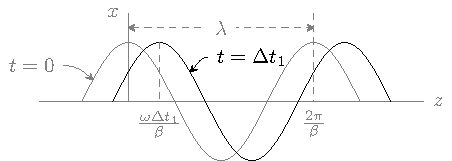
\includegraphics{figWaveMovingRightWithTime}
\caption{وقت $t=0$ اور $t=t_1$ پر خلاء میں موج کا مقام۔}
\label{شکل_موج_وقت_کے_ساتھ_مثبت_چلتی_موج}
\end{figure}


موج کی مساوات  میں \عددیء{\alpha=0} تصور کرتے ہوئے اسے وقت \عددیء{t=0} پر شکل \حوالہ{شکل_موج_وقت_کے_ساتھ_مثبت_چلتی_موج} میں ہلکی سیاہی سے دکھایا گیا ہے۔یہاں دھیان رہے کہ شکل میں \عددیء{z} محدد کو افقی دکھایا گیا ہے۔جیسے آپ دیکھ سکتے ہیں \عددیء{t=0} پر موج کی دو آپس میں قریبی چوٹیاں \عددیء{z=0} اور \عددیء{z=\tfrac{2\pi}{\beta}} پر پائی جاتی ہیں۔دو آپس میں قریبی چوٹیوں کے درمیان فاصلے کو \اصطلاح{طول موج}\فرہنگ{طول موج}\فرہنگ{موج!طول}\حاشیہب{wavelength}\فرہنگ{wavelength} پکارا اور \عددیء{\lambda} سے ظاہر کیا جاتا ہے۔یوں اس موج کی طول موج
\begin{align}\label{مساوات_موج_زاویائی_مستقل_اور_طول_موج_الف}
\lambda=\frac{2\pi}{\beta}
\end{align}
ہے جس سے
\begin{align}\label{مساوات_موج_زاویائی_مستقل_اور_طول_موج_ب}
\beta=\frac{2\pi}{\lambda}
\end{align}
لکھا جا سکتا ہے جو انتہائی اہم نتیجہ ہے۔

موج کی مساوات ہی کو وقت \عددیء{t=\Delta t_1} پر شکل \حوالہ{شکل_موج_وقت_کے_ساتھ_مثبت_چلتی_موج} میں دوبارہ گاڑھی سیاہی میں بھی دکھایا گیا ہے۔آپ دیکھ سکتے ہیں کہ اس دورانیے میں موج نے دائیں جانب یعنی \عددیء{z} بڑھنے کی طرف حرکت کی ہے۔یوں صاف ظاہر ہے کہ یہ موج وقت کے ساتھ مثبت \عددیء{z} جانب حرکت کر رہی ہے۔ دورانیہ \عددیء{\Delta t_1} میں موج کی چوٹی نے \عددیء{\tfrac{\omega \Delta t_1}{\beta}} فاصلہ طے کیا ہے لہٰذا موج کے رفتار کو
\begin{align}\label{مساوات_موج_رفتار_اور_تعدد}
v=\frac{\Delta z}{\Delta t}=\frac{\omega \Delta t_1}{\beta} \frac{1}{\Delta t_1}=\frac{\omega}{\beta}
\end{align}
لکھا جا سکتا ہے۔

مساوات \حوالہ{مساوات_موج_زاویائی_مستقل_اور_طول_موج_ب} کو  مساوات \حوالہ{مساوات_موج_رفتار_اور_تعدد} میں پر کرنے سے
\begin{align}
v=f \lambda
\end{align}
حاصل ہوتا ہے جو \عددیء{\lambda} طول موج  اور \عددیء{f} تعدد رکھنے والے موج کی رفتار \عددیء{v} دیتی ہے۔

مساوات \حوالہ{مساوات_موج_کوسائن_مثبت_موج} میں مساوات \حوالہ{مساوات_موج_رفتار_اور_تعدد} استعمال کرتے ہوئے
\begin{align}
E_x=E_0 e^{-\alpha z} \cos \left[ \omega \left(t-\frac{z}{v} \right)\right]
\end{align}
حاصل ہوتا ہے جسے مساوات \حوالہ{مساوات_موج_رفتار_اور_تعدد} اور مساوات \حوالہ{مساوات_موج_زاویائی_مستقل_اور_طول_موج_ب} کی مدد سے
\begin{align}
E_x=E_0 e^{-\alpha z} \cos \left(\omega  t-\frac{2 \pi z}{\lambda}\right)
\end{align}
بھی لکھا جا سکتا ہے۔

موج کی رفتار کو مساوات \حوالہ{مساوات_موج_کوسائن_مثبت_موج} سے دوبارہ حاصل کرتے ہیں۔اس مساوات کے تحت کسی بھی لمحہ \عددیء{t} پر موج کی چوٹی اس مقام پر ہو گی جہاں
\begin{align*}
\omega t -\beta z=0
\end{align*}
ہو۔چونکہ رفتار \عددیء{\tfrac{\dif z}{\dif t}} کو کہتے ہیں لہٰذا اس مساوات کے تفرق
\begin{align*}
\omega \dif t-\beta \dif z=0
\end{align*}
سے رفتار
\begin{align}
v=\frac{\dif z}{\dif t}=\frac{\omega}{\beta}
\end{align}
حاصل ہوتی ہے۔

\begin{figure}
\centering
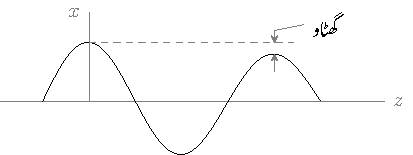
\includegraphics{figWaveAttenuation}
\caption{موج چلتے ہوئے آہستہ آہستہ کمزور ہوتی رہتی ہے۔}
\label{شکل_موج_کمزوری}
\end{figure}

شکل \حوالہ{شکل_موج_کمزوری} میں \عددیء{\alpha} کو صفر تصور نہیں کیا گیا ہے۔جیسا کہ آپ دیکھ سکتے ہیں، ایسی صورت میں موج کی چوٹی، \عددیء{z} کے ساتھ بتدریج گھٹتی  ہے لہٰذا \عددیء{{\alpha=\SI{0.001}{\neper \per \meter}}} کی صورت میں \عددیء{\SI{1}{\kilo \meter}} کے فاصلے پر موج کی چوٹی، ابتدائی چوٹی کے \عددیء{\tfrac{e^{-1}}{e^{-0}}=0.368} گنا رہ گئی ہو گی جہاں ابتدائی چوٹی \عددیء{z=0} پر لی گئی ہے۔

برقی موج \عددیء{\kvec{E}_{s}} سے مساوات \حوالہ{مساوات_موج_میکس_ویل_دوری_سمتیہ_شکل_الف}
\begin{align*}
\nabla \times \kvec{E}_{s}=-j \omega \mu \kvec{H}_{s}
\end{align*}
 کی مدد سے مقناطیسی موج با آسانی حاصل ہوتی ہے۔مساوات \حوالہ{مساوات_موج_مثبت_زیڈ_جانب_سمتی} استعمال کرتے ہوئے مندرجہ بالا مساوات سے
\begin{align*}
-\gamma E_0 e^{-\gamma z} \ay=-j \omega \mu \kvec{H}_s
\end{align*}
یا
\begin{align*}
\kvec{H}_s=\frac{\gamma}{j \omega \mu} E_0 e^{-\gamma z} \ay
\end{align*}
حاصل ہوتا ہے جس میں مساوات \حوالہ{مساوات_موج_حرکی_مستقل_الف} سے مثبت \عددیء{\gamma} کی قیمت پر کرنے سے
\begin{gather}
\begin{aligned}\label{مساوات_موج_مقناطیسی_جزو}
\kvec{H}_s&=\sqrt{\frac{\sigma +j \omega \epsilon}{j \omega \mu}} E_0 e^{-\gamma z} \ay\\
&=\frac{E_0}{\eta} e^{-\gamma z}\ay
\end{aligned}
\end{gather}
ملتا ہے جہاں دوسرے قدم پر
\begin{align}\label{مساوات-موج_قدرتی_رکاوٹ}
\eta =\sqrt{\frac{j \omega \mu}{\sigma +j \omega \epsilon}}
\end{align}
لکھی\حاشیہد{یونانی حروف تہجی \عددیء{\eta} ایٹا پڑھا جاتا ہے۔}\حاشیہب{\عددیء{\eta}، eta} گئی ہے۔

مساوات \حوالہ{مساوات_موج_مثبت_زیڈ_جانب_سمتی} کی غیر سمتی صورت یعنی \عددیء{E_{xs}=E_0e^{-\gamma z}} کو مساوات \حوالہ{مساوات_موج_مقناطیسی_جزو} کے غیر سمتی صورت یعنی \عددیء{H_{ys}=\tfrac{E_0}{\eta}e^{-\gamma z}} سے تقسیم کرتے ہوئے
\begin{align}
\frac{E_{xs}}{H_{ys}}=\eta
\end{align}
ملتا ہے۔

یہاں ذرہ رک کر ایک برقی دور پر غور کرتے ہیں۔منبع برقی دباو \عددیء{V_0 \cos (\omega t -\psi)} جسے دوری سمتیہ \عددیء{V_0 e^{-j\psi}} لکھا جا سکتا ہے کے ساتھ سلسلہ وار مزاحمت \عددیء{R}، امالہ \عددیء{L} اور کپیسٹر \عددیء{C} جڑے ہیں جن کی رکاوٹ \عددیء{Z}
\begin{align*}
Z=R+j\left( \omega L -\frac{1}{\omega C}\right)=R+jX=\abs{Z} e^{j \theta_Z}=\abs{Z}\phase{\theta_Z}
\end{align*}
لکھی جا سکتی ہے  جہاں \عددیء{\omega L > \tfrac{1}{\omega C}} کی صورت میں \عددیء{X} مثبت ہو گا جبکہ \عددیء{\omega L < \tfrac{1}{\omega C}} کی صورت میں یہ منفی ہو گا۔مزید \عددیء{\omega L = \tfrac{1}{\omega C}} کی صورت میں دور خالص مزاحمتی رکاوٹ پیش کرے گا اور \عددیء{\theta_Z=0} ہو گا۔اس دور میں برقی رو دوری سمتیہ کی مدد سے
\begin{align*}
I_s=\frac{V_s}{Z_s}=\frac{V_0 e^{-j\psi}}{\abs{Z}e^{j \theta_Z}}=\frac{V_0}{\abs{Z}}e^{-j(\psi+\theta_Z)}
\end{align*}
حاصل ہوتا ہے جس سے
\begin{align*}
i=\frac{V_0}{\abs{Z}}\cos \left(\omega t -\psi-\theta_Z \right)
\end{align*}
لکھا جا سکتا ہے۔برقی دباو اور برقی رو ایک ہی تعدد رکھتے ہیں البتہ ان میں زاویائی فاصلہ \عددیء{\theta_Z} پایا جاتا ہے۔مثبت \عددیء{X} کی صورت میں برقی رو اس زاویائی فاصلے کے برابر برقی دباو کے پیچھے رہتی ہے جبکہ منفی \عددیء{X} کی صورت میں برقی رو اس زاویائی فاصلے کے برابر برقی دباو کے آگے رہتی ہے۔ہم دیکھتے ہیں کہ برقی دباو اور برقی رو کی شرح
\begin{align*}
\frac{V_s}{I_s}=\abs{Z} e^{j \theta_Z}=Z
\end{align*}
کے برابر ہے جسے رکاوٹ کہتے ہیں۔

آئیں اب دوبارہ امواج کی بات کریں۔برقی موج کو اس مثال کے برقی دباو کی جگہ اور مقناطیسی موج کو مثال کے رو کی جگہ رکھتے ہوئے آپ دیکھیں گے کہ دونوں مسائل ہوبہو یکساں ہیں۔اسی وجہ سے  برقی موج \عددیء{E_{xs}} اور مقناطیسی موج \عددیء{H_{ys}} کی شرح \عددیء{\eta}،  \اصطلاح{قدرتی رکاوٹ}\فرہنگ{قدرتی رکاوٹ}\فرہنگ{رکاوٹ!قدرتی}\حاشیہب{intrinsic impedance}\فرہنگ{intrinsic impedance} کہلاتی ہے۔بالکل برقی رکاوٹ کی طرح قدرتی رکاوٹ حقیقی یا خیالی اور یا مخلوط عدد ہو سکتا ہے۔قدرتی رکاوٹ کی اکائی اوہم \عددیء{\si{\ohm}} ہے۔

مساوات \حوالہ{مساوات_موج_مقناطیسی_جزو} سے مقناطیسی موج
\begin{align}\label{مساوات_موج_عمومی_مقناطیسی}
H_y=\frac{E_0 e^{-\alpha z}}{\abs{\eta}} \cos \left(\omega t - \beta z -\theta_{\eta} \right)
\end{align}
لکھی جائے گی جہاں قدرتی رکاوٹ کو
\begin{align}
\eta=\abs{\eta} e^{j \theta_{\eta}}
\end{align}
لکھا گیا۔

مساوات \حوالہ{مساوات_موج_کوسائن_مثبت_موج} کے تحت برقی میدان \عددیء{x} محدد کے متوازی ہے جبکہ مساوات \حوالہ{مساوات_موج_عمومی_مقناطیسی} کے تحت مقناطیسی میدان \عددیء{y} محدد کے متوازی ہے لہٰذا یہ میدان  آپس میں ہر وقت عمودی رہتے ہیں۔اس کے علاوہ دونوں امواج \عددیء{z} سمت میں حرکت کر رہے ہیں۔یوں میدان کی سمت اور حرکت کی سمت بھی آپس میں عمودی ہیں۔ایسے امواج جن میں میدان کی سمت اور حرکت کی سمت عمودی ہوں \اصطلاح{عرضی امواج}\فرہنگ{عرضی موج}\فرہنگ{موج!عرضی}\حاشیہب{transverse waves}\فرہنگ{transverse waves} کہلاتے ہیں۔پانی کی سطح پر لہریں بھی عرضی امواج ہوتے ہیں۔اسی طرح رسی کو کھینچ کر رکھتے ہوئے اسے جھٹکے  سے ہلانے سے  رسی میں عرضی موج پیدا ہوتی ہے۔ 

\جزوحصہ{خالی خلاء میں امواج کی خاصیت}
خالی خلاء میں \عددیء{\sigma=0}، \عددیء{\mu_R=1} اور \عددیء{\epsilon_R=1}  ہیں لہٰذا مساوات \حوالہ{مساوات_موج_حرکی_مستقل_الف} سے مثبت حرکی مستقل
\begin{align*}
\gamma=\sqrt{j \omega \mu_R \mu_0  \left(\sigma +j \omega \epsilon_R \epsilon_0 \right)}=j \omega \sqrt{\mu_0 \epsilon_0}
\end{align*}
حاصل ہوتا ہے جس سے
\begin{align*}
\alpha&=0\\
\beta&=\omega \sqrt{\mu_0 \epsilon_0}
\end{align*}
حاصل ہوتے ہیں۔یوں خالی خلاء میں برقی و مقناطیسی امواج کی رفتار، جسے روایتی طور پر \عددیء{c} سے ظاہر کیا جاتا ہے،  مساوات \حوالہ{مساوات_موج_رفتار_اور_تعدد} سے
\begin{align}
c=\frac{\omega}{\beta}=\frac{1}{\sqrt{\mu_0 \epsilon_0}}
\end{align}
حاصل ہوتی ہے جس کی قیمت
\begin{align*}
c=\frac{1}{\sqrt{4 \times \pi \times 10^{-7} \times 8.854 \times 10^{-12}}}&=\SI{2.99e8}{\meter \per \second} \\
&\approx \SI{3e8}{\meter \per \second}
\end{align*}
ہے۔

مساوات \حوالہ{مساوات-موج_قدرتی_رکاوٹ} سے خالی خلاء کی قدرتی رکاوٹ
\begin{align*}
\eta =\sqrt{\frac{j \omega \mu_R \mu_0}{\sigma +j \omega \epsilon_R \epsilon_0}}=\sqrt{\frac{\mu_0}{\epsilon_0}}
\end{align*}
حاصل ہوتی ہے۔قدرتی رکاوٹ کی قیمت حاصل کرنے کی خاطر ہم \عددیء{\tfrac{1}{4\pi \epsilon_0}=9\times 10^9} سے \عددیء{\epsilon_0=\tfrac{1}{36\pi 10^9}} لکھتے ہوئے
\begin{align}
\eta=120 \pi \approx \SI{377}{\ohm}
\end{align}
حاصل کرتے ہیں۔یوں خالی خلاء میں کسی بھی لمحے، کسی بھی نقطے پر برقی میدان کی قیمت اس نقطے پر مقناطیسی میدان کے \عددیء{377} گنا ہو گی۔

حرکی مستقل اور قدرتی رکاوٹ کی قیمتیں استعمال کرتے ہوئے خالی خلاء میں متحرک موج کے میدان
\begin{align*}
E_x&=E_0 \cos \left[\omega \left( t -\frac{z}{c} \right)\right]\\
H_y&=\frac{E_0}{120 \pi} \cos \left[ \omega \left( t -\frac{z}{c} \right) \right]
\end{align*}
لکھے جائیں گے۔آپ دیکھ سکتے ہیں کہ دونوں میدان ہم زاویہ ہیں۔یوں کسی بھی نقطے پر بڑھتے برقی میدان کی صورت میں اس نقطے پر مقناطیسی میدان بھی بڑھتا ہے۔ان مساوات کے تحت امواج بالکل سیدھے حرکت کرتے ہیں اور نا وقت اور نا ہی فاصلے کے ساتھ ان کی طاقت میں کسی قسم کی کمی رونما ہوتی ہے۔یہی وجہ ہے کہ کائنات کے دور ترین کہکشاوں سے ہم تک برقی و مقناطیسی امواج پہنچتی ہیں اور ہمیں رات کے چمکتے اور خوبصورت تارے نظر آتے ہیں۔

%=========================
\ابتدا{مشق}
بے تار ذرائع ابلاغ میں \عددیء{\SI{36000}{\kilo \meter}} کی اونچائی پر پرواز کرتے مصنوعی سیارے اہم کردار ادا کرتے ہیں۔یہ سیارے زمین کے اوپر ایک ہی نقطے پر آویزاں نظر آتے ہیں۔ان سیاروں سے زمین کے قریبی نقطے تک برقی اشارہ کتنی دیر میں پہنچے گا۔

جواب:\عددیء{\SI{0.12}{\second}}
\انتہا{مشق}
%=========================

\جزوحصہ{خالص ذو برق میں امواج کی خاصیت}
خالص ذو برقی سے مراد ایسا ذو برق ہے جس میں متحرک برقی و مقناطیسی امواج کی توانائی ضائع نہیں ہوتی۔خالص ذو برق میں \عددیء{\sigma=0} جبکہ اس کا جزوی مقناطیسی مستقل \عددیء{\mu_R} اور جزوی برقی مستقل \عددیء{\epsilon_R}  ہے لہٰذا مساوات \حوالہ{مساوات_موج_حرکی_مستقل_الف} سے مثبت حرکی مستقل
\begin{align*}
\gamma=j \omega \sqrt{\mu \epsilon }
\end{align*}
حاصل ہوتا ہے جس سے
\begin{align*}
\alpha&=0\\
\beta&=\omega \sqrt{\mu \epsilon}
\end{align*}
حاصل ہوتے ہیں۔یوں خالی خلاء میں برقی و مقناطیسی امواج کی رفتار  مساوات \حوالہ{مساوات_موج_رفتار_اور_تعدد} سے
\begin{align}
v=\frac{\omega}{\beta}=\frac{1}{\sqrt{\mu_R \mu_0 \epsilon_R \epsilon_0}}=\frac{c}{\sqrt{\mu_R \epsilon_R}}
\end{align} 
حاصل ہوتی ہے جہاں \عددیء{\tfrac{1}{\sqrt{\mu_0 \epsilon_0}}} کو خالی خلاء میں روشنی کی رفتار \عددیء{c} لکھا گیا ہے۔چونکہ ذو برق میں \عددیء{\mu_R \epsilon_R > 1} ہے  لہٰذا ذو برق میں روشنی کی رفتار خالی خلاء میں روشنی کے رفتار سے کم ہو گی۔خالی خلاء میں روشنی کی رفتار اس کی زیادہ سے زیادہ رفتار ہے۔

موج کی رفتار اور تعدد سے طول موج
\begin{align}
\lambda=\frac{v}{f}=\frac{c}{f \sqrt{\mu_R \epsilon_R}}=\frac{\lambda_0}{\sqrt{\mu_R \epsilon_R}}
\end{align}
حاصل ہوتی ہے جہاں خالی خلاء کے طول موج کو \عددیء{\lambda_0} لکھا گیا ہے۔اس مساوات سے ذو برق میں روشنی کی رفتار کم ہونے کی وجہ سامنے آتی ہے۔چونکہ \عددیء{\mu_R \epsilon_R >1} ہے لہٰذا ذو برق میں طول موج کم ہو جاتا ہے جس سے روشنی کی رفتار کم ہو جاتی ہے۔


مساوات \حوالہ{مساوات-موج_قدرتی_رکاوٹ} سے ذو برقی کی  قدرتی رکاوٹ
\begin{align*}
\eta =\sqrt{\frac{\mu}{\epsilon}}=\sqrt{\frac{\mu_0}{\epsilon_0}}\sqrt{\frac{\mu_R}{\epsilon_R}}= \eta_0 \sqrt{\frac{\mu_R}{\epsilon_R}}
\end{align*}
حاصل ہوتی ہے جہاں خالی خلاء کی قدرتی رکاوٹ کو \عددیء{\eta_0} لکھا گیا ہے۔

یوں ذو برق میں امواج کے مساوات
\begin{align}
E_x&=E_0 \cos (\omega t -\beta z)\\
H_y&=\frac{E_0}{\eta} \cos (\omega t -\beta z)
\end{align}
ہیں۔

%==================
\ابتدا{مثال}
پانی کے لئے \عددیء{\mu_R=1}، \عددیء{\epsilon_R=80} اور \عددیء{\sigma=0} لیتے ہوئے \عددیء{\SI{300}{\mega \hertz}} تعدد کے برقی و مقناطیسی امواج کی رفتار، طول موج اور قدرتی رکاوٹ حاصل کریں۔ برقی میدان \عددیء{\SI{50}{\milli \volt \per \meter}} ہونے کی صورت میں برقی اور مقناطیسی امواج کے مساوات لکھیں۔ہم \عددیء{\sigma=0} لیتے ہوئے درحقیقت پانی میں توانائی کے ضیاع کو نظرانداز کر رہے ہیں۔

حل:
\begin{align*}
v=\frac{c}{\sqrt{\mu_R \epsilon_R}}=\frac{3 \times 10^8}{\sqrt{80}}=\SI{0.3354e8}{\meter \per \second}\\
\lambda=\frac{v}{f}=\frac{0.3354 \times 10^8}{300 \times 10^6}=\SI{11.18}{\centi\meter}
\end{align*}
ہیں جبکہ خالی خلاء میں \عددیء{\lambda=\SI{1}{\meter}} ہے۔بقایا مستقل
\begin{align*}
\beta=\frac{2\pi}{\lambda}=\SI{56.2}{\radian \per \meter}
\end{align*}
اور
\begin{align*}
\eta=\eta_0 \sqrt{\frac{\mu_R}{\epsilon_R}}=\frac{377}{80}=\SI{42.15}{\ohm}
\end{align*}
ہیں۔امواج کے مساوات
\begin{align*}
E_x&=0.05 \cos (6\pi 10^8 t -56.2 z)\\
H_y&=\frac{0.05}{42.15} \cos (6\pi 10^8 t -56.2 z)=0.00119 \cos (6\pi 10^8 t -56.2 z)
\end{align*}
ہیں۔
\انتہا{مثال}
%===================
\ابتدا{مشق}
کتاب کے آخر میں مختلف اشیاء کے مستقل دئے گئے ہیں۔انہیں استعمال کرتے ہوئے  عمبر میں \عددیء{\SI{5.6}{\giga\hertz}} اور \عددیء{\SI{10}{\milli \ampere \per \meter}} طول کے مقناطیسی میدان پر عمبر میں مندرجہ ذیل حاصل کریں۔
\begin{itemize}
\item
موج کی رفتار،
\item
طول موج،
\item
زاویائی مستقل،
\item
قدرتی رکاوٹ،
\item
برقی میدان کا طول۔
\end{itemize} 

جوابات:\عددیء{\SI{1.82e8}{\meter \per \second}}، \عددیء{\SI{32.6}{\centi\meter}}، \عددیء{\SI{192.76}{\radian \per \meter}}، \عددیء{\SI{229.3}{\ohm}} اور \عددیء{\SI{2.29}{\volt \per \meter}}
\انتہا{مشق}
%===================

\جزوحصہ{موج کی طاقت گھٹاتے ذو برقی میں امواج}

